\chapter{Aplicaciones de Amplificadores Operacionales}

\hspace{10pt}
Dado el diagrama circuital de la figura \ref{lab3_1}:

\begin{enumerate}
	\item Diseñar la Etapa 1 para obtener una onda cuadrada en $v_a$ de
	frecuencia $f_o = 100Hz$ y una amplitud pico a pico de 14,8V, con un
	único ajuste en $R_4$. Elija $R_3$ de modo que la corriente de
	salida del AO esté comprendida entre 4 y 5ma. Realizar las
	mediciones y observaciones necesarias de las tensiones $v_a$ y
	$v_c$, mediante el uso de un osciloscopio.
	\item En la Etapa 2, elegir $R_6$ para obtener $v_b$ (pico a pico) de
	aproximadamente 2V. Observar y medir dicha tensión con el
	osciloscopio. Observar la tensión $v_e$, sacar conclusiones.
	\item Con los valores de diseño elegidos en las etapas
	anteriores hallar teóricamente la forma de onda de  la tensión de
	salida $v_o$. Verificar dicho desarrollo con lo observado en el
	laboratorio.
	\item Realizar un informe escrito completo de la
	práctica de Laboratorio.
	
\end{enumerate}


\begin{figure}[h]
	\centering
	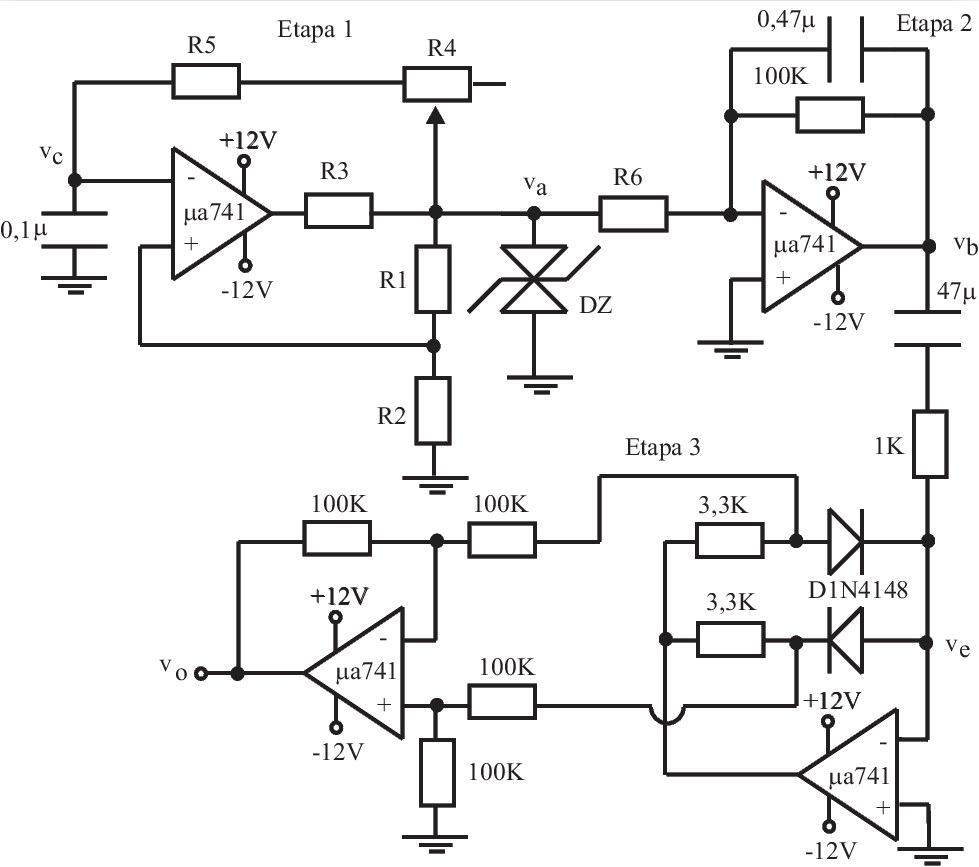
\includegraphics[width=0.8\linewidth]{figuras/lab3_1.png}\\
	\caption{}\label{lab3_1}
\end{figure}